
\subsection{Bending machine}
\begin{figure}[h]
    \centering
    \includegraphics[width=\textwidth]{figures/bending-machine.png}
    \caption{\hyperref[acro:AMADA]{AMADA} Bending Machine 1) Marker 2) Bending station 3) Laser height 4) Laser monitoring 5) \hyperref[acro:TFT]{TFT} Touch screen}
    \label{fig:bending_machine}
\end{figure}

\subsection{Robot Unit}

The robot unit consists of three assemblies: a base, a robot and a gripper (Figure \ref{fig:kr1410}).

\begin{figure}[h]
    \centering
    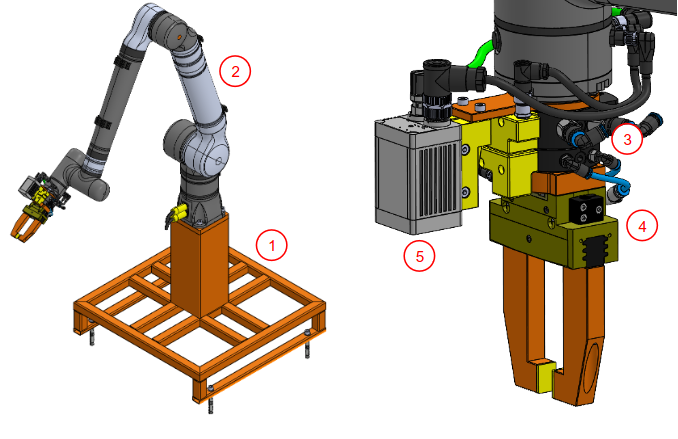
\includegraphics[width=\textwidth]{4. Hardware Integration/4.1 Installation and Configuration/kr1410.png}
    \caption{Components of the robot unit: 1) robot base; 2) robot from kassow robots; 3) manual quick-change system; 4) pneumatic parellel gripper; 5) camera system}
    \label{fig:kr1410}
\end{figure}

The base is a simple welded construction made of steel. The choice of steel material ensures that the base has
sufficient dead weight so that it can be transported together with the robot and gripper using a pallet
truck without the risk of tipping over. During operation, the robot unit is fixed to the floor with four M12
screws. The robot used is a 7-axis robot from Kassow Robots. This fulfills the requirements defined in
the first work packages. The gripper is a pneumatic parallel gripper with a manual quick-change
system. The gripper was selected according to payload, gripping force and opening width. The
opening width is the dominant selection criterion here, as the gripper must be able to grip both the thin
sheets with thicknesses of around 1 to 3 mm and the handle on the drawers with a width of 15 mm. An
electric gripper was also considered, as the power supply could have been provided via the cable
already integrated in the robot. Due to the higher costs, the double height and the weight, a pneumatic
gripper was chosen.




The manual quick-change system makes it possible to exchange different gripper
designs in a short time and without increased effort if required for a sheet metal part type. Sheet metal
part is folded into something like a box. For this, it is technically sensible or necessary to use a
vacuum gripper.
This means that collision-free gripping is not possible with a parallel gripper after the last bend. The
quick-change system also has an electric and pneumatic power feed-through, which ensures simple,
user-friendly changeover.



Furthermore, a camera system is installed on the robot itself. This is used to determine the relative
position between the robot unit and the sheet pickup station, bending machine and storage shelf using the markers
and between the robot unit and the sheet metal part (when it is first made available at the
sheet pickup station or is gripped) using features on the sheet metal part.

The robotic system consists of a manipulator from kassow robots with pneumatic parallel grippers as the end-effector.
Pneumatic gripper is controlled by PLC. \hyperref[acro:VISOR]{VISOR\textsuperscript{\textregistered}} camera is also mounted on the tool-IO which is used for robotic perception.



\subsection{Unloading station}
    Figure 7 shows the elementary components of this station.
    A room gantry with a working area of 400 x 1000 x 250 mm is to be used for destacking. All electronic
    components such as fuses, power supply units, etc. of the entire mobile robot unit, i.e. not just those of
    the unloading station, are installed in several control cabinets below the room gantry. This allows the
    removal station to be used more flexibly later on different sheet metal bending machines. The same is
    planned for the pneumatic components such as switching valves, pressure regulators, pressure
    gauges, etc. Due to the flexibility and the space still available, the robot's control cabinet will also be
    equipped by Kassow Robots with integrated. As with the robot unit, different grippers (vacuum grippers, magnetic grippers, etc.) can be
    installed very quickly using a manual quick-change system, depending on the type of sheet metal part.
    After the gripper has unstacked a raw sheet, it is transferred to a pneumatic 180° swivel unit, which in
    turn is equipped with one or more pneumatic parallel grippers (depending on the sheet size). From
    there, the raw sheet is finally picked up by the robot unit described in the previous subsection after the
    exact position has been determined with the camera on the robot. In order to achieve reliable and
    precise positioning, an LED panel is installed as background lighting below the swivel unit. An HMI
    control unit is installed for the operation (start, pause, stop, etc.) of the entire mobile robot unit and as
    a source of information about relevant process values, such as the remaining time until the deposit
    box is completely filled or the removal station is empty. The protective fence in Figure 1 is flush with
    the removal station, but contains a recess so that the HMI can be used at all times.

    Similar to the storage box, the raw sheets are stored on a pull-out drawer (Figure 8). This also consists
    of a universal basic construction and an individual perforated grid plate. Depending on the type of
    sheet metal part, the blanks can be stacked on this perforated grid plate. The sheet metal parts can be
    held in place by means of sheet metal brackets that are screwed to the plate. Telescopic rails are also
    used here. Because the drawer does not have to be opened by a robot, but only by a person, rails with
    integrated locking mechanisms can be used. Pulling out the drawer ensures ergonomically simple
    filling. The drawer position is monitored using a position switch.